\section{System Evaluation}
\label{sec:syseval}
We evaluate our system's generalisability on six benchmark tasks (Table \ref{table:task-list}) and show how taught actions can be reused for complex tasks.
The tasks involved manipulating different object types on four marked positions with both claw and suction grippers.
We take the Blocksworld domain (\cite{slaney2001blocks}) for building and rebuilding stacked objects (Tasks 1-4) and an elaborate version of the Tower of Hanoi problem with different object types to build a `house' (Tasks 5\&6).
Instead of disks, we decided to use different object types (ROOF, CUBE, BASE), where BASE corresponds to the largest disk, followed by CUBE and BASE.
The rules for stacking different objects still apply (\eg BASE cannot be stacked on top of ROOF or CUBE).
However, to demonstrate the generalisation of actions to diverse tasks, additional constraints are added as objects cannot be all manipulated in the same way, \ie using different grippers.
The order of the tasks was given with increasing complexity, requiring the user to modify existing actions or teach new actions from scratch.
% to show reusability of more and more complex tasks we use the Tower of Hanoi problem with different number of disks, to show its applicability in real-world, we take an assembly task.
% The most common tasks for industrial robots are assembly, packaging, and material handling (such as polishing etc.) \footnote{https://blog.robotiq.com/the-3-most-common-tasks-delegated-to-robots-in-manufacturing}.
%Picking, Packing and Palletizing – Most products are handled multiple times prior to final shipping. Robotic picking and packaging increases speed and accuracy along with lowering production costs \footnote{https://www.jabil.com/insights/blog-main/ten-popular-industrial-robot-applications.html}
% Assembly and packaging tasks require prior planning in order to complete a task efficiently.
%Thus, we take an assembly task to build a ..and a packaging task with.


\begin{table}[h]
	\begin{center}
		\caption{Benchmark tasks for the system evaluation. Three different pick-and-place actions using (claw and suction grippers) were programmed.}
		\label{table:task-list}
		%\begin{center}
		\begin{tabular}{clll}
			\# & Task Goal & Pick-and-place action\\ \hline
			1 & Build tower with 3 CUBES & claw from top \\
			2 & Build tower with 4 CUBES & claw from top \\
			3 & Rebuild Task 2 on a different position & claw from top \\
			4 & Build tower and move (w/o disassembly) & claw from top \& claw from side \\
			5 & Build house with BASE, CUBE, ROOF & claw from top \& suction from top \\
			6 & Rebuild Task 5 on a different position & claw from top \& suction from top \\
			% 5 & Assembly & P\&p with turning/orienting \\
			% 6 & Packaging & P\&p with pushing to save space \\
		\end{tabular}
	\end{center}
\end{table}

\subsection{Protocol}
The tasks were programmed with the most efficient teaching strategy of minimising the number of actions created and generalising them by changing the action properties (as described in Section \ref{sec:generalisation}).
Depending on the given task and involved objects, the experimenter decided what manipulation action needed to be taught.
Only one planning problem was created and reused for all tasks by redetecting the objects in the initial state and changing the goal states.
When the generated plan was incorrect, the debug menu on the GUI was used to determine the changes to be made to generalise the actions.
A task was considered completed when the generated plan was correct and the robot successfully executed it in real-time.
As the mental model saved the latest object positions after an action execution, Tasks 3 and 6 were continued from the preceding tasks and did not require redetecting the initial states. 
%reusing the problem with the latest saved mental model allowed them to overcome the limitation to detect stacked objects.


\subsection{Results}
We programmed three manipulation actions for the six benchmark tasks, which involved demonstrating pick-and-place actions with claw and suction grippers from the \textit{top} and from the \textit{side}.
Actions were generalised by changing parameter types (\eg from CUBE or POSITION to ELEMENT) or adding preconditions or effects which were not inferred automatically.
For pick-and-place actions from the top, `obj is clear' was added as a precondition (Task 1-3), while it was not included when picking an object from the side to allow moving a pile of objects (Task 4).
For actions involving the claw gripper, the precondition `obj is thin' was added so that the robot would only use it on ROOF and CUBE objects, similarly `is flat' for the suction gripper (Task 5\&6).
The `is stackable' condition was used for the Tower of Hanoi as an equivalent to the rule `larger objects cannot be placed on top of smaller ones'.
The robot was able to generate plans for all tasks and executed them in real time at least twice (\fig{fig:filmstrip}).\footnote{A subset of the task executions can be seen on \url{https://youtu.be/NgaTPG8dZwg}}
Note that the taught actions can be reused for a diverse range of problems beyond the six benchmark tasks.
This evaluation shows the generalisability of our system, allowing us to teach primitive actions by demonstration and reuse them with a task planner to solve more complex problems.

\begin{figure*}[h]
	\centering
	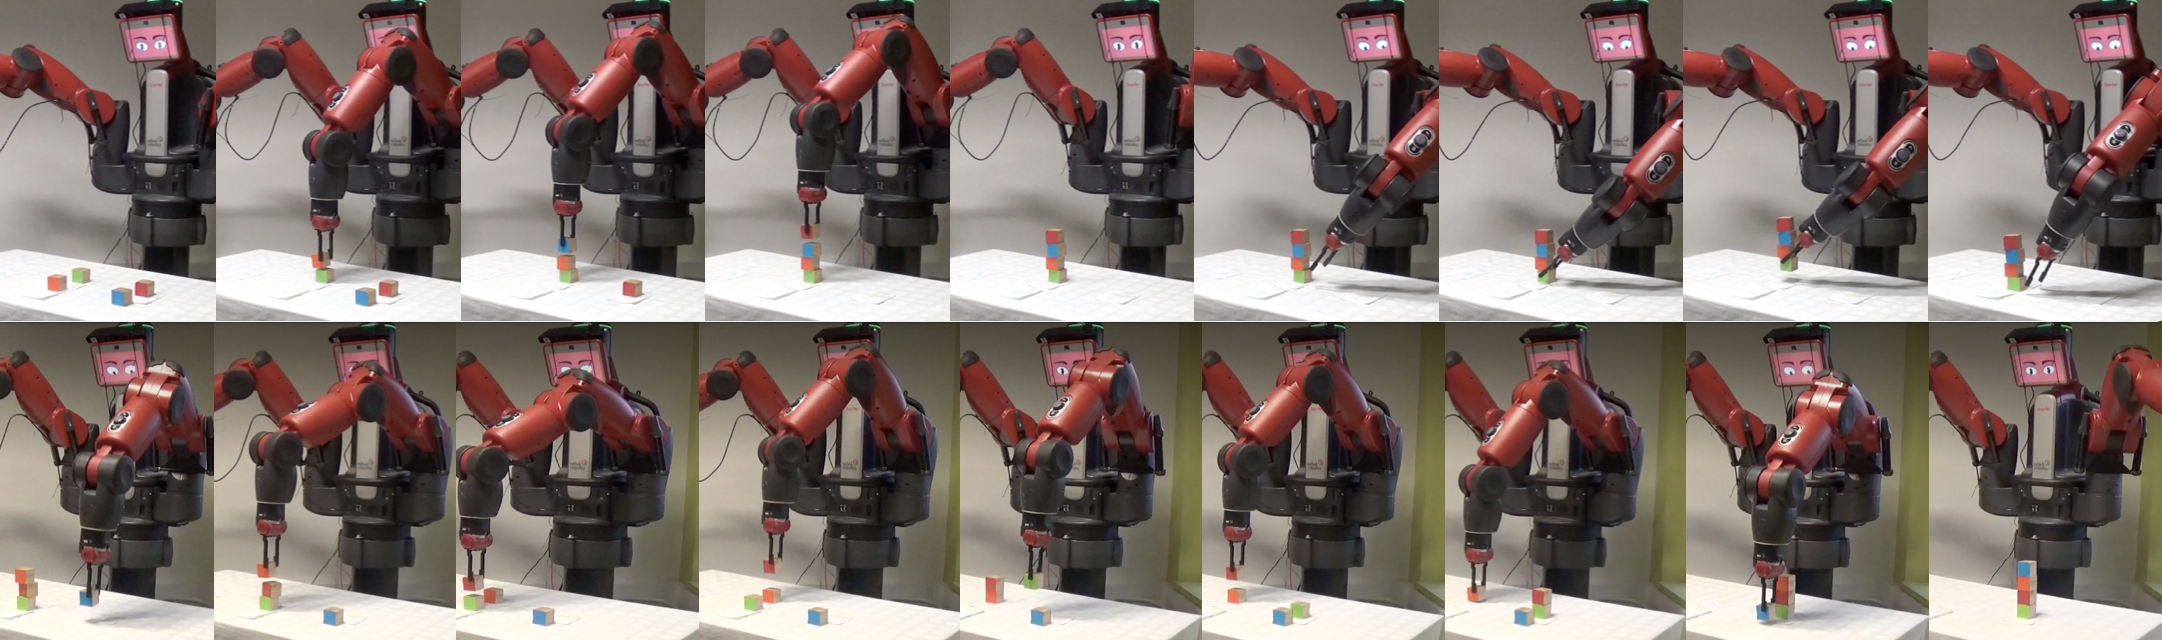
\includegraphics[width=\linewidth]{figures/filmstrip.png}
	\caption{Snapshots from the executions of the system evaluation (Tasks 3\&4) showing a claw grip from the top and the side.}
	\label{fig:filmstrip}
\end{figure*}